
L'objectif de cette partie est d'exprimer le flux radiatif $q$~[W/m²] sortant de chaque face solide, afin de prendre en compte le rayonnement dans les transferts thermiques. Plusieurs phénomènes sont à prendre en compte simultanément dans un problème radiatif: l'émission, la transmission, l'absorption et la réflexion. Plusieurs hypothèses retenues permettent de simplifier la mise en équation du système.

\subsection{Formulation du problème}
La modélisation du problème radiatif repose sur les hypothèses suivantes :

\begin{enumerate}
    \item \textbf{Transparence du fluide} : le milieu séparant les surfaces n'absorbe, n'émet ni ne réfléchit de rayonnement. Cela revient à considérer que les photons sont transportés sans interaction dans le milieu.
    
    \item \textbf{Opacité des surfaces solides} : la transmission à travers les surfaces est négligée. Le rayonnement incident, aussi appelé irradiance ($G$~[W/m²]), est donc soit réfléchi, soit absorbé. Les coefficients de réflexion et d'absorption sont ainsi complémentaires à 1 pour chaque longueur d'onde :
    \begin{equation}
        \forall \lambda, \quad \rho_{\lambda} + \alpha_{\lambda} = 1
    \end{equation}
    
    \item \textbf{Surfaces grises et diffuses} : les coefficients d'absorption et d'émission sont égaux et ne dépendent que de la température, $\alpha(T) = \epsilon(T)$.
    
    \item \textbf{Uniformité de la température par surface} : chaque surface est supposée isotherme.
\end{enumerate}

Ces hypothèses permettent d'introduire la radiosité $J$~[W/m²] (voir Figure~\ref{fig:radio}), qui correspond à l'ensemble de l'énergie rayonnée quittant une surface. Elle s'écrit comme la somme de la puissance émissive de la surface $E_i$~[W/m²] et de la fraction réfléchie de l'irradiance $\rho_i G_i$~[W/m²] :

\begin{equation}
    \forall \vec{r}_i \in \text{Surface}_i, \quad J_i(\vec{r_i}) = \epsilon_i \sigma \big(T_i)\big)^4 + \rho_i G_i(\vec{r_i})
    \label{def:radiosite}
\end{equation} 

avec $\epsilon_i$ (resp. $\rho_i$) l'émissivité (resp. la réflectivité) de la surface $i$, $\sigma$ la constante de Stefan-Boltzmann et $T_i$ la température de la surface $i$ à la position $\vec{r}_i$. Le flux radiatif en surface s'écrit alors, par le bilan suivant :

\begin{equation}
    \forall \vec{r}_i \in \text{Surface}_i,\quad q_i(\vec{r}_i) =  J(\vec{r}_i)  - G(\vec{r}_i) 
    \label{eq:qr}
\end{equation}

Une dernière hypothèse concerne le caractère diffus de l'irradiance : $G_{\lambda, i}(\lambda, \theta, \varphi)$ est supposée indépendante de $\lambda$, $\theta$ et $\varphi$, comme l'illustre la Figure~\ref{fig:diffus}.

\begin{minipage}{0.45\textwidth}
    \centering
    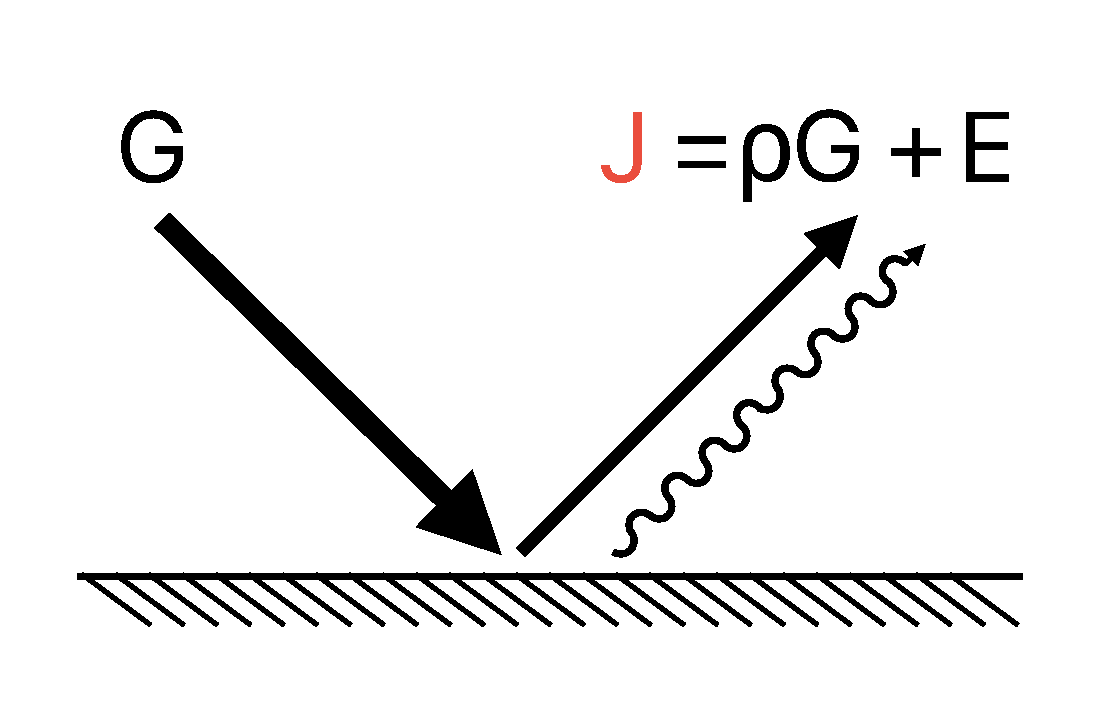
\includegraphics[width=0.9\textwidth]{PICTURES/radiosite.pdf}
    \captionof{figure}{Échanges radiatifs considérés dans le problème}
    \label{fig:radio}
\end{minipage}
\hfill
\begin{minipage}{0.45\textwidth}
    \centering
    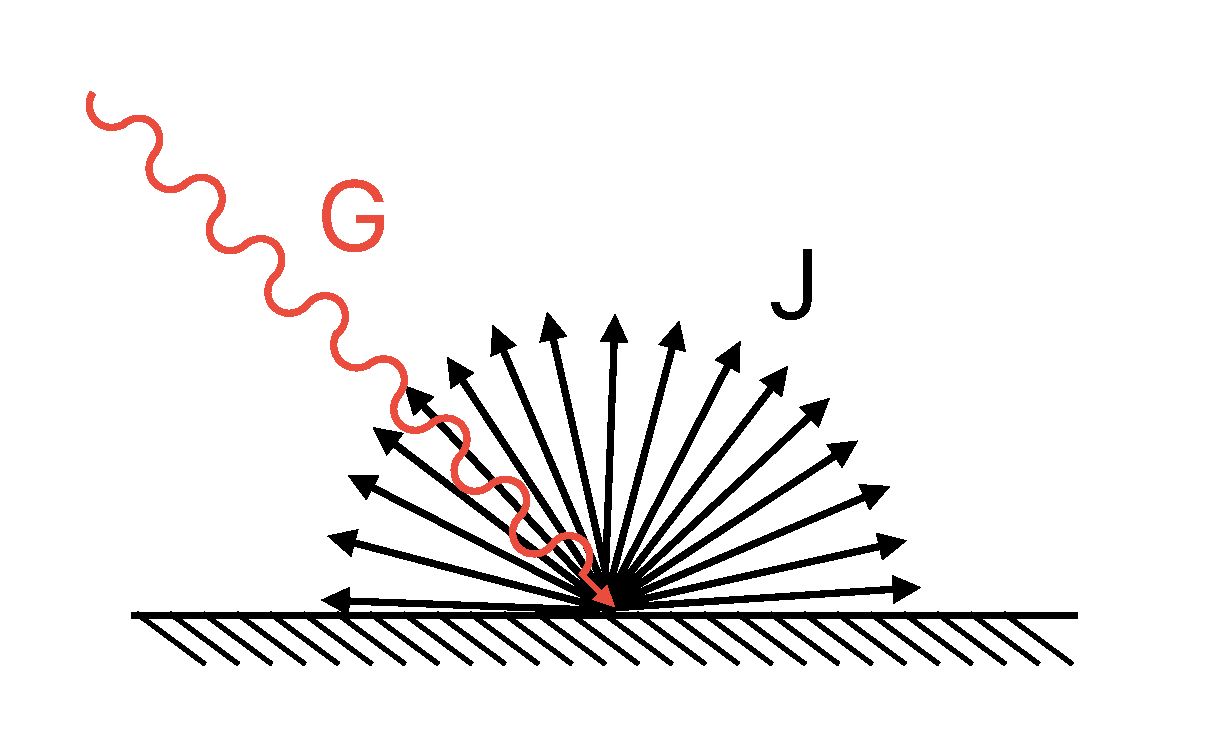
\includegraphics[width=0.9\textwidth]{PICTURES/diffus.pdf}
    \captionof{figure}{Illustration de l'hypothèse de réflexion et émission diffuse}
    \label{fig:diffus}
\end{minipage}




Pour finir, l’irradiance est exprimée conformément à la Figure \ref{fig:fij_schema} en fonction des radiosités sous la forme : 
\begin{equation}
    \forall i \in [1, n], \forall \vec{r_i} \in A_i , \quad G_i(\vec{r_i}) = \sum_{j = 1}^{n} \frac{1}{\pi} \int_{A_j} d^2(\vec{r_j})J_j(\vec{r_j})\bigg[\frac{cos(\theta_{ij})cos(\theta_{ji})}{||\vec{r_i}-\vec{r_j}||^2} \chi{(\vec{r_i},\vec{r_j})}\bigg] 
    \label{def:irra}
\end{equation}
Avec $\chi$ la fonction de visibilité qui vaut 1 si les points $\vec{r_i}$ et $\vec{r_j}$ sont visibles l'un de l'autre, et 0 sinon.
\begin{figure}[h]
    \centering
    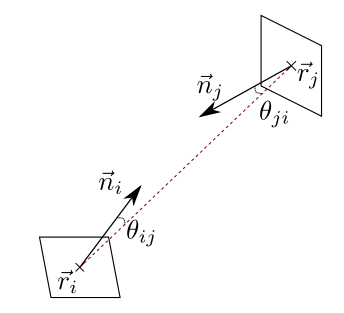
\includegraphics[width = 0.3\linewidth]{PICTURES/FIJ.png}
    \caption{Illustration des notations géométriques introduites à l'Équation \ref{def:irra}}
    \label{fig:fij_schema}
\end{figure}






